\section{Interfaccia utente}
\label{sec:userInterface}
L'interfaccia utente è il luogo d'incontro tra il sistema distribuito e l'utilizzatore finale. In questo elaborato di tesi, come detto in precedenza, l'utente che vuole utilizzare e controllare i risultati del sistema distribuito deve utilizzare un qualsiasi browser e digitare l'indirizzo web del server di Blockchain explorer. L'utente dunque da qualsiasi tipo di dispositivo può accedere alla home page del portale ed iniziare ad utilizzare il sistema.
\\L'immagine \ref{fig:homePage} mostra la prima schermata che l'utente visualizza quando accede al portale.
\begin{figure}[H]
	\centering
	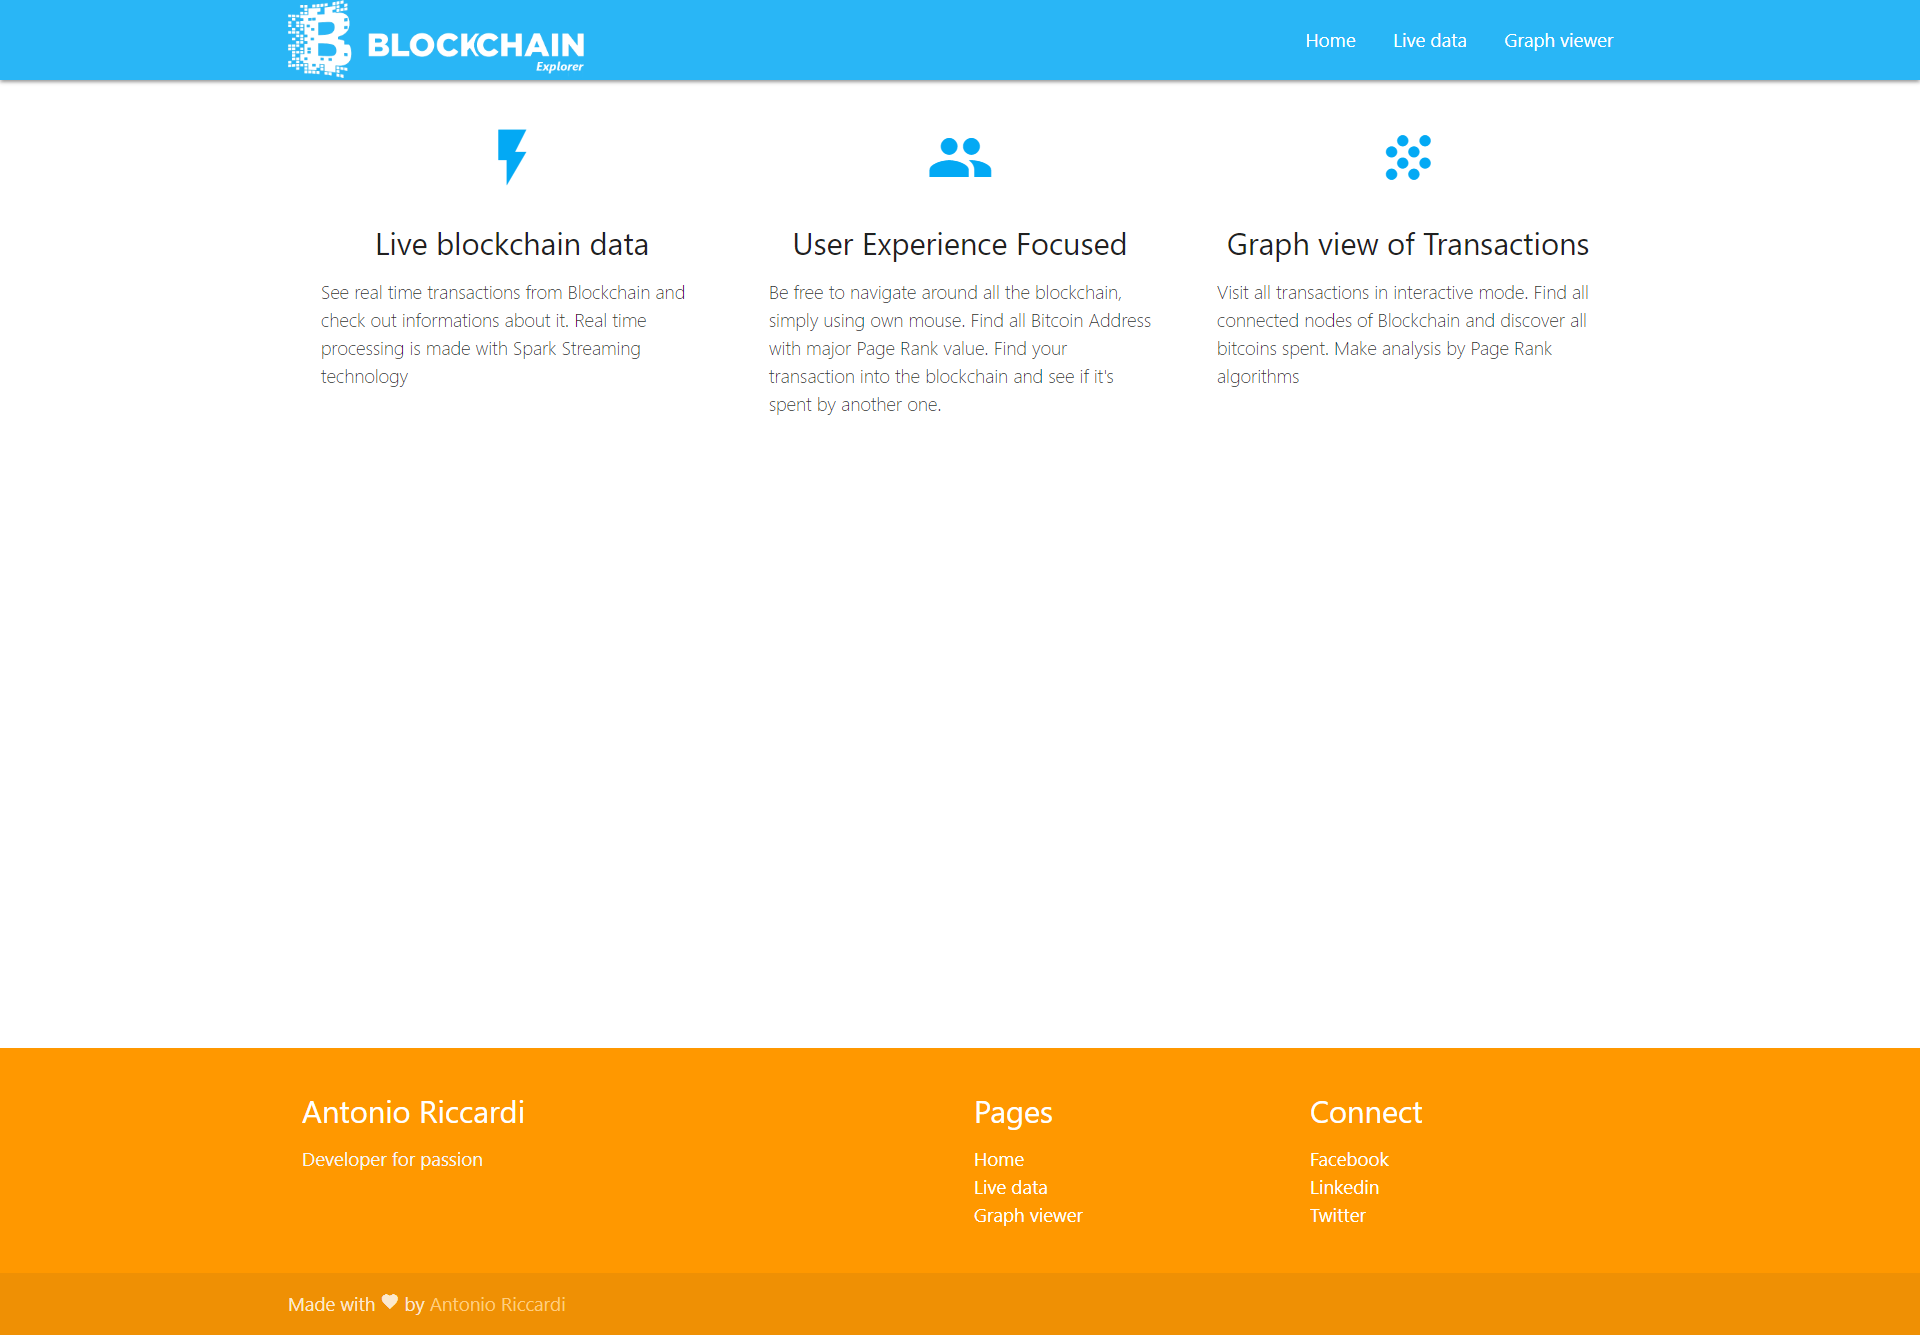
\includegraphics[width=\textwidth, height=0.70\textheight]{images/homePage.png}
	\caption{Home page Blockchain Explorer.}
	\label{fig:homePage}
\end{figure}
Nella prima pagina mostrata agli utenti, sono descritte brevemente tutte le funzionalità offerte dal sito. Per accedere a queste funzionalità il sito mette a disposizione due menù: il primo nella parte alta ed il secondo nel footer. Entrambi i menù forniscono i link alle pagine per visualizzare i dati in real time (Live Data) ed il grafo delle transazioni con i relativi page rank (Graph viewer).
\\La ricezione dei dati in real time è mostrata in figura \ref{fig:transactionsBE} ed accessibile dai menù tramite la voce \textit{Live Data}. Questa funzionalità quindi, permette di controllare le ultime transazioni avvenute sulla Blockchain, in maniera tabellare, senza dover ricaricare la pagina.
\begin{figure}[H]
	\centering
	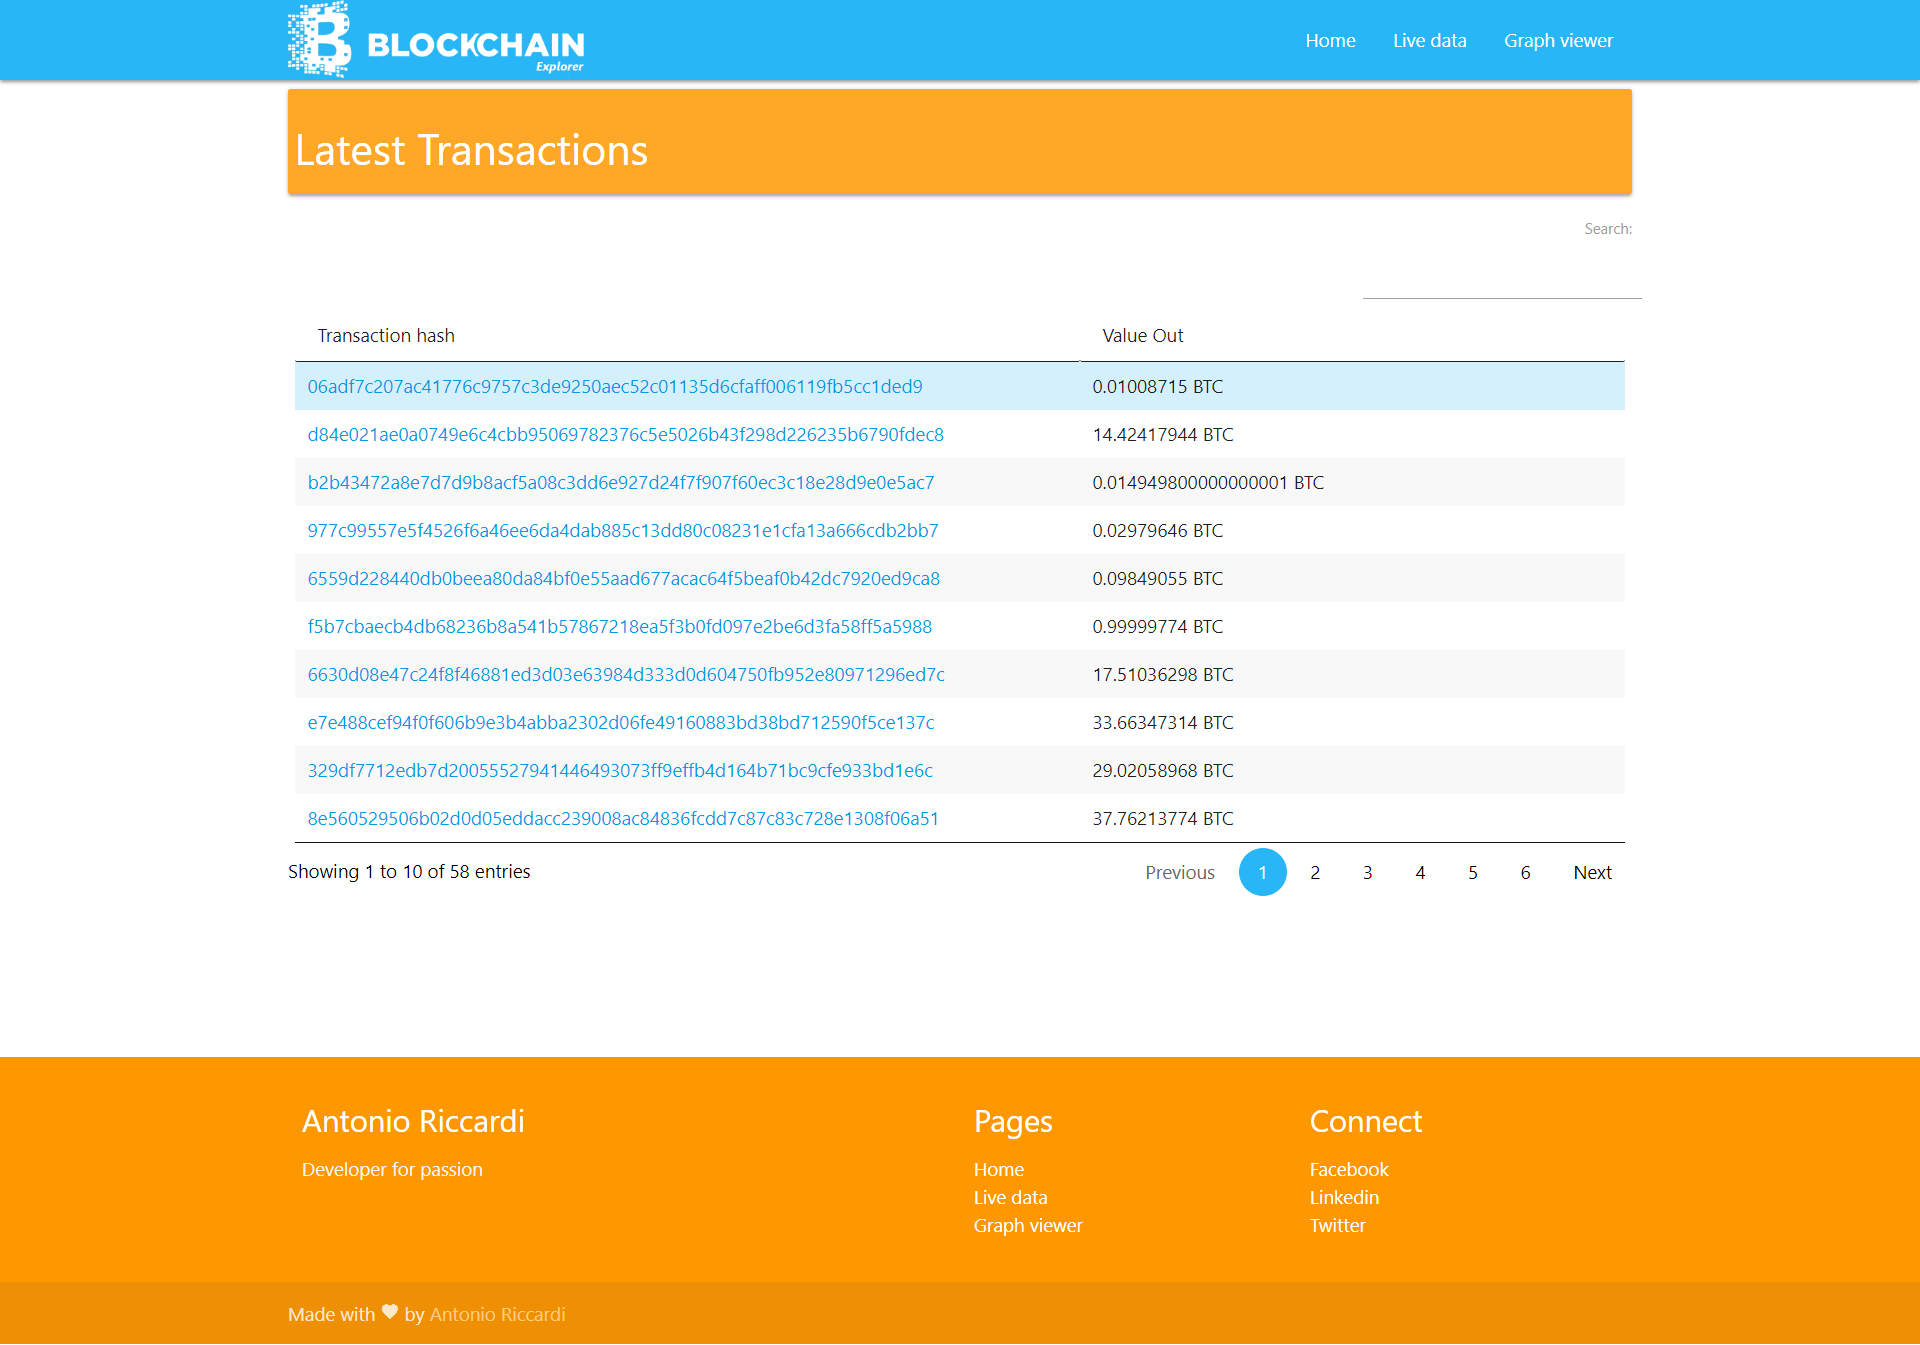
\includegraphics[width=\textwidth, height=0.70\textheight]{images/lastTransaction.png}
	\caption{Elenco ultime transazioni.}
	\label{fig:transactionsBE}
\end{figure}
Live data, inoltre offre la possibilità di mostrare il dettaglio di una transazione semplicemente selezionando l'hash dalla tabella. Questa operazione apre una nuova scheda del browser, che mostra le informazioni di dettaglio e la ricostruzione grafica della transazione selezionata. L'immagine \ref{fig:detailBE} mostra una scheda di dettaglio per la transazione con hash \textbf{3099179a36d5b50b9992d89c5be8e9dfb1561ac3a7110c95bd0e049ff8cfe1d7}
\begin{figure}[H]
	\centering
	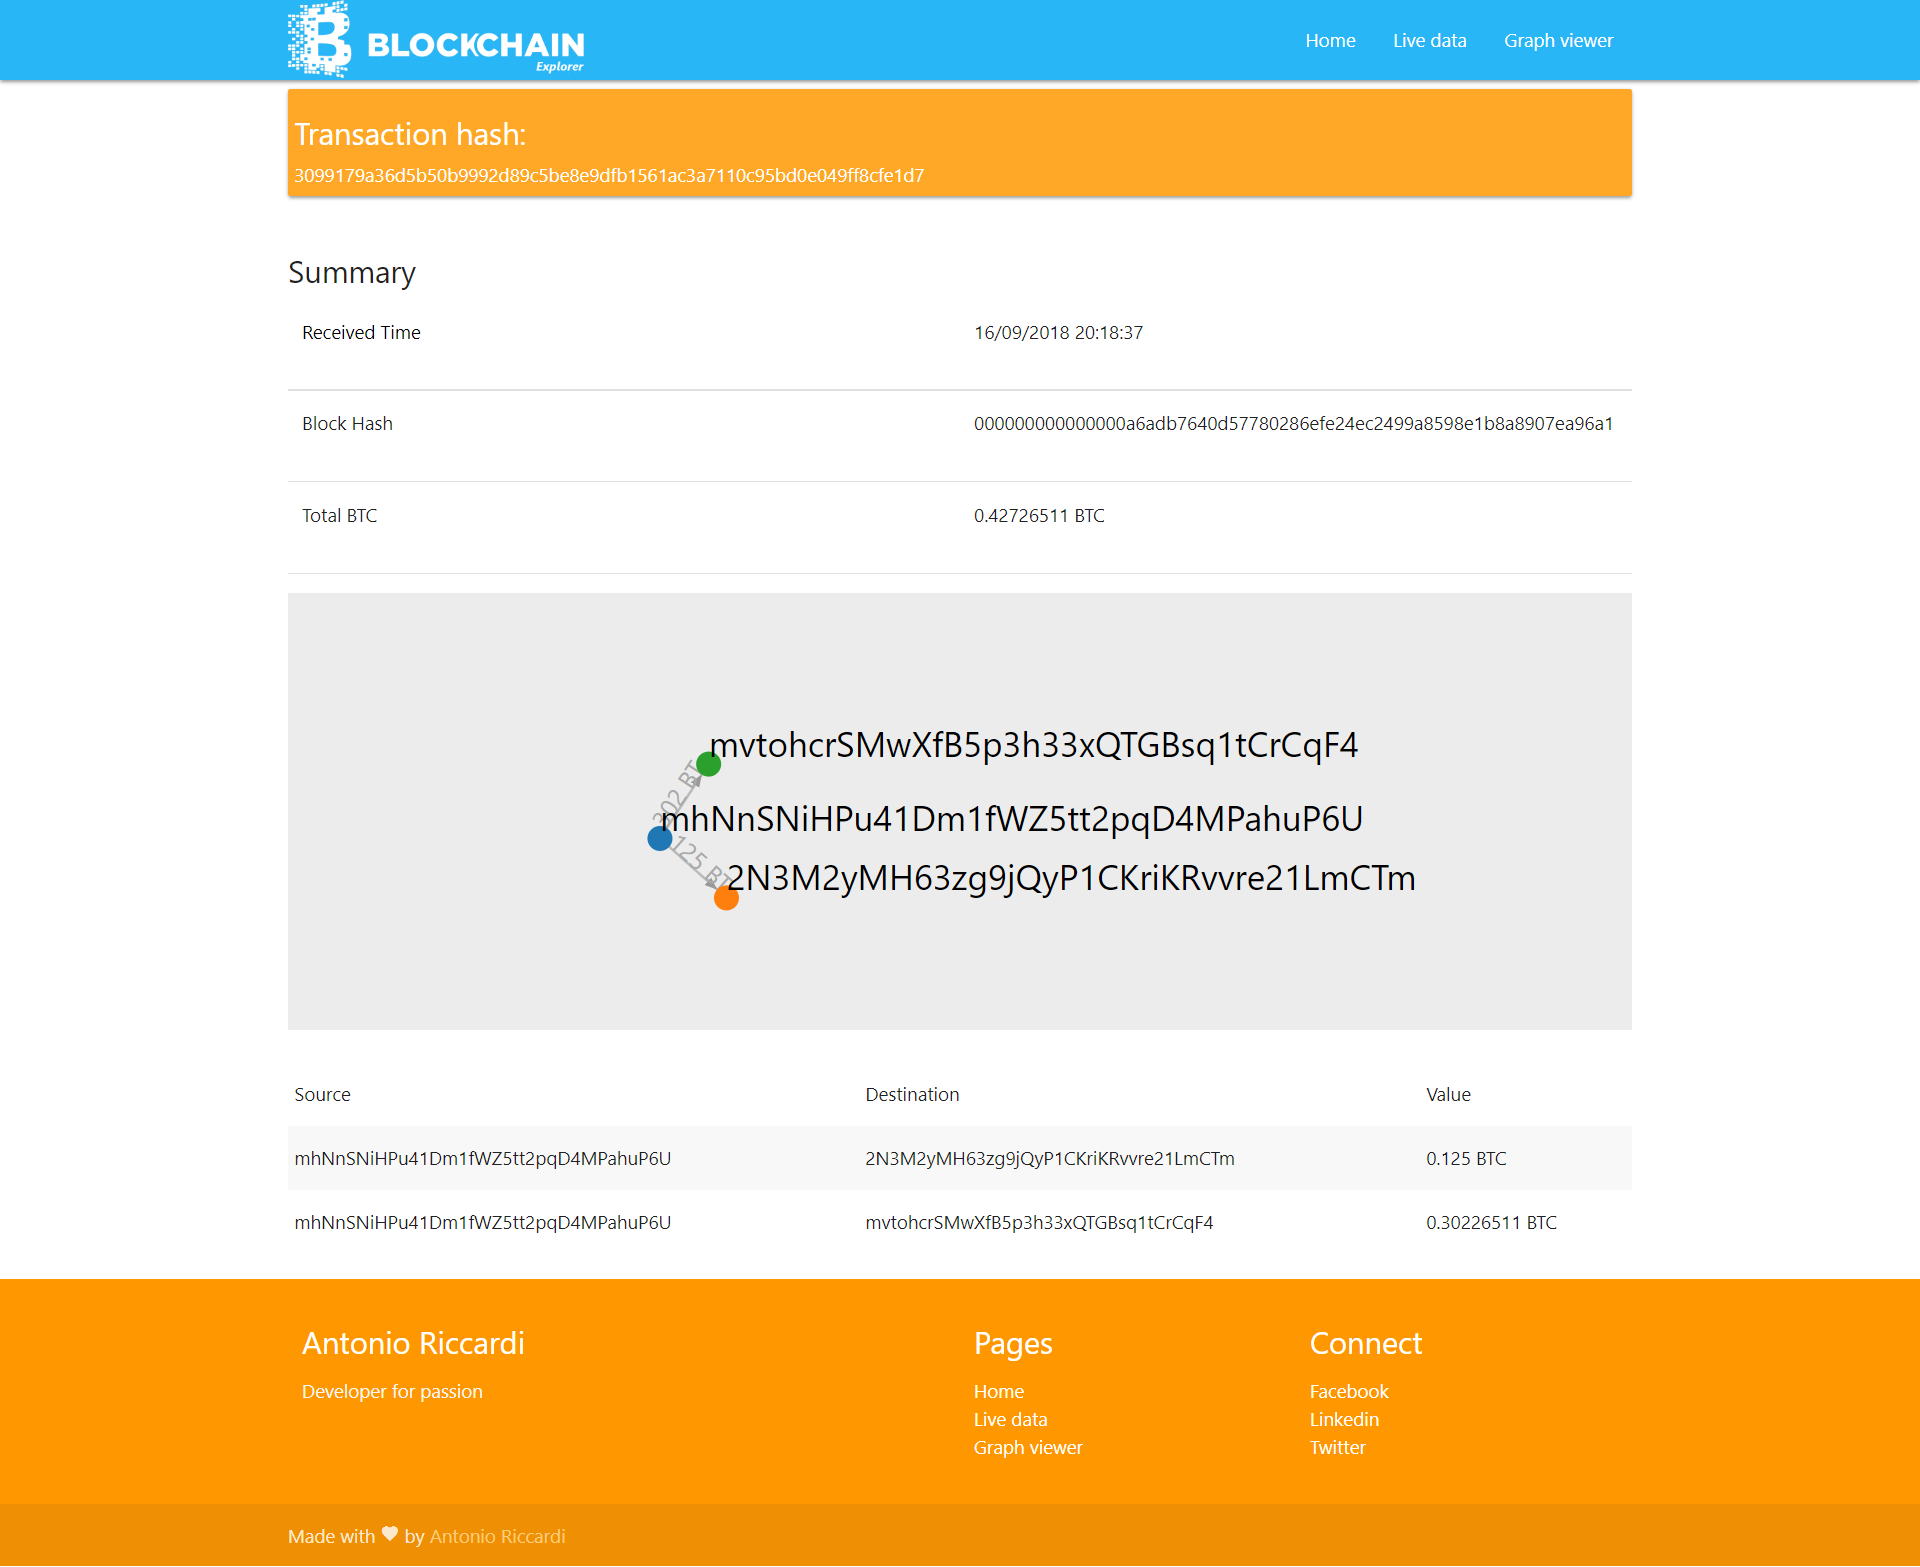
\includegraphics[width=\textwidth, height=0.70\textheight]{images/infoTransaction2.png}
	\caption{Dettaglio transazione.}
	\label{fig:detailBE}
\end{figure}
In particolare la figura sopra citata aggiunge informazioni relative al timestamp della transazione, l'hash del blocco di appartenenza e il totale dei Bitcoin spesi in questa transazione. Infine, è presente un grafico che raffigura lo scambio di bitcoin ed una tabella che descrive l'andamento di tale transazione. Nell'immagine \ref{fig:detailBE} è possibile notare che indirizzo hash \textbf{mhNnSNiHPu41Dm1fWZ5tt2pqD4MPahuP6U} ha avviato la transazione inviando 0.125 BTC al destinatario \textbf{2N3M2yMH63zg9jQyP1CKriKRvvre21LmCTm} ed i restanti 0.30226511 BTC all'hash \textbf{mvtohcrSMwXfB5p3h33xQTGBsq1tCrCqF4}; in virtù del protocollo Bitcoin, il quale stabilisce che il resto di una transazione genera un nuovo hash e quindi un nuovo input per una successiva transazione, uno dei due hash citati precedentemente si presuppone essere il resto di questa transazione e che quindi appartenga alla stessa persona che ha avviato la transazione. \footnote{Questa transazione può essere verificata sul sito ufficiale di \textit{BlockCyhper} all'indirizzo \url{https://live.blockcypher.com/btc-testnet/tx/3099179a36d5b50b9992d89c5be8e9dfb1561ac3a7110c95bd0e049ff8cfe1d7/}}
\\Altra funzionalità molto importate fornita dall'applicazione è la possibilità di controllare lo stato della blockchain. Questa particolare funzione è accessibile dai menù cliccando sulla voce \textit{Graph viewer}.
\begin{figure}[H]
	\centering
	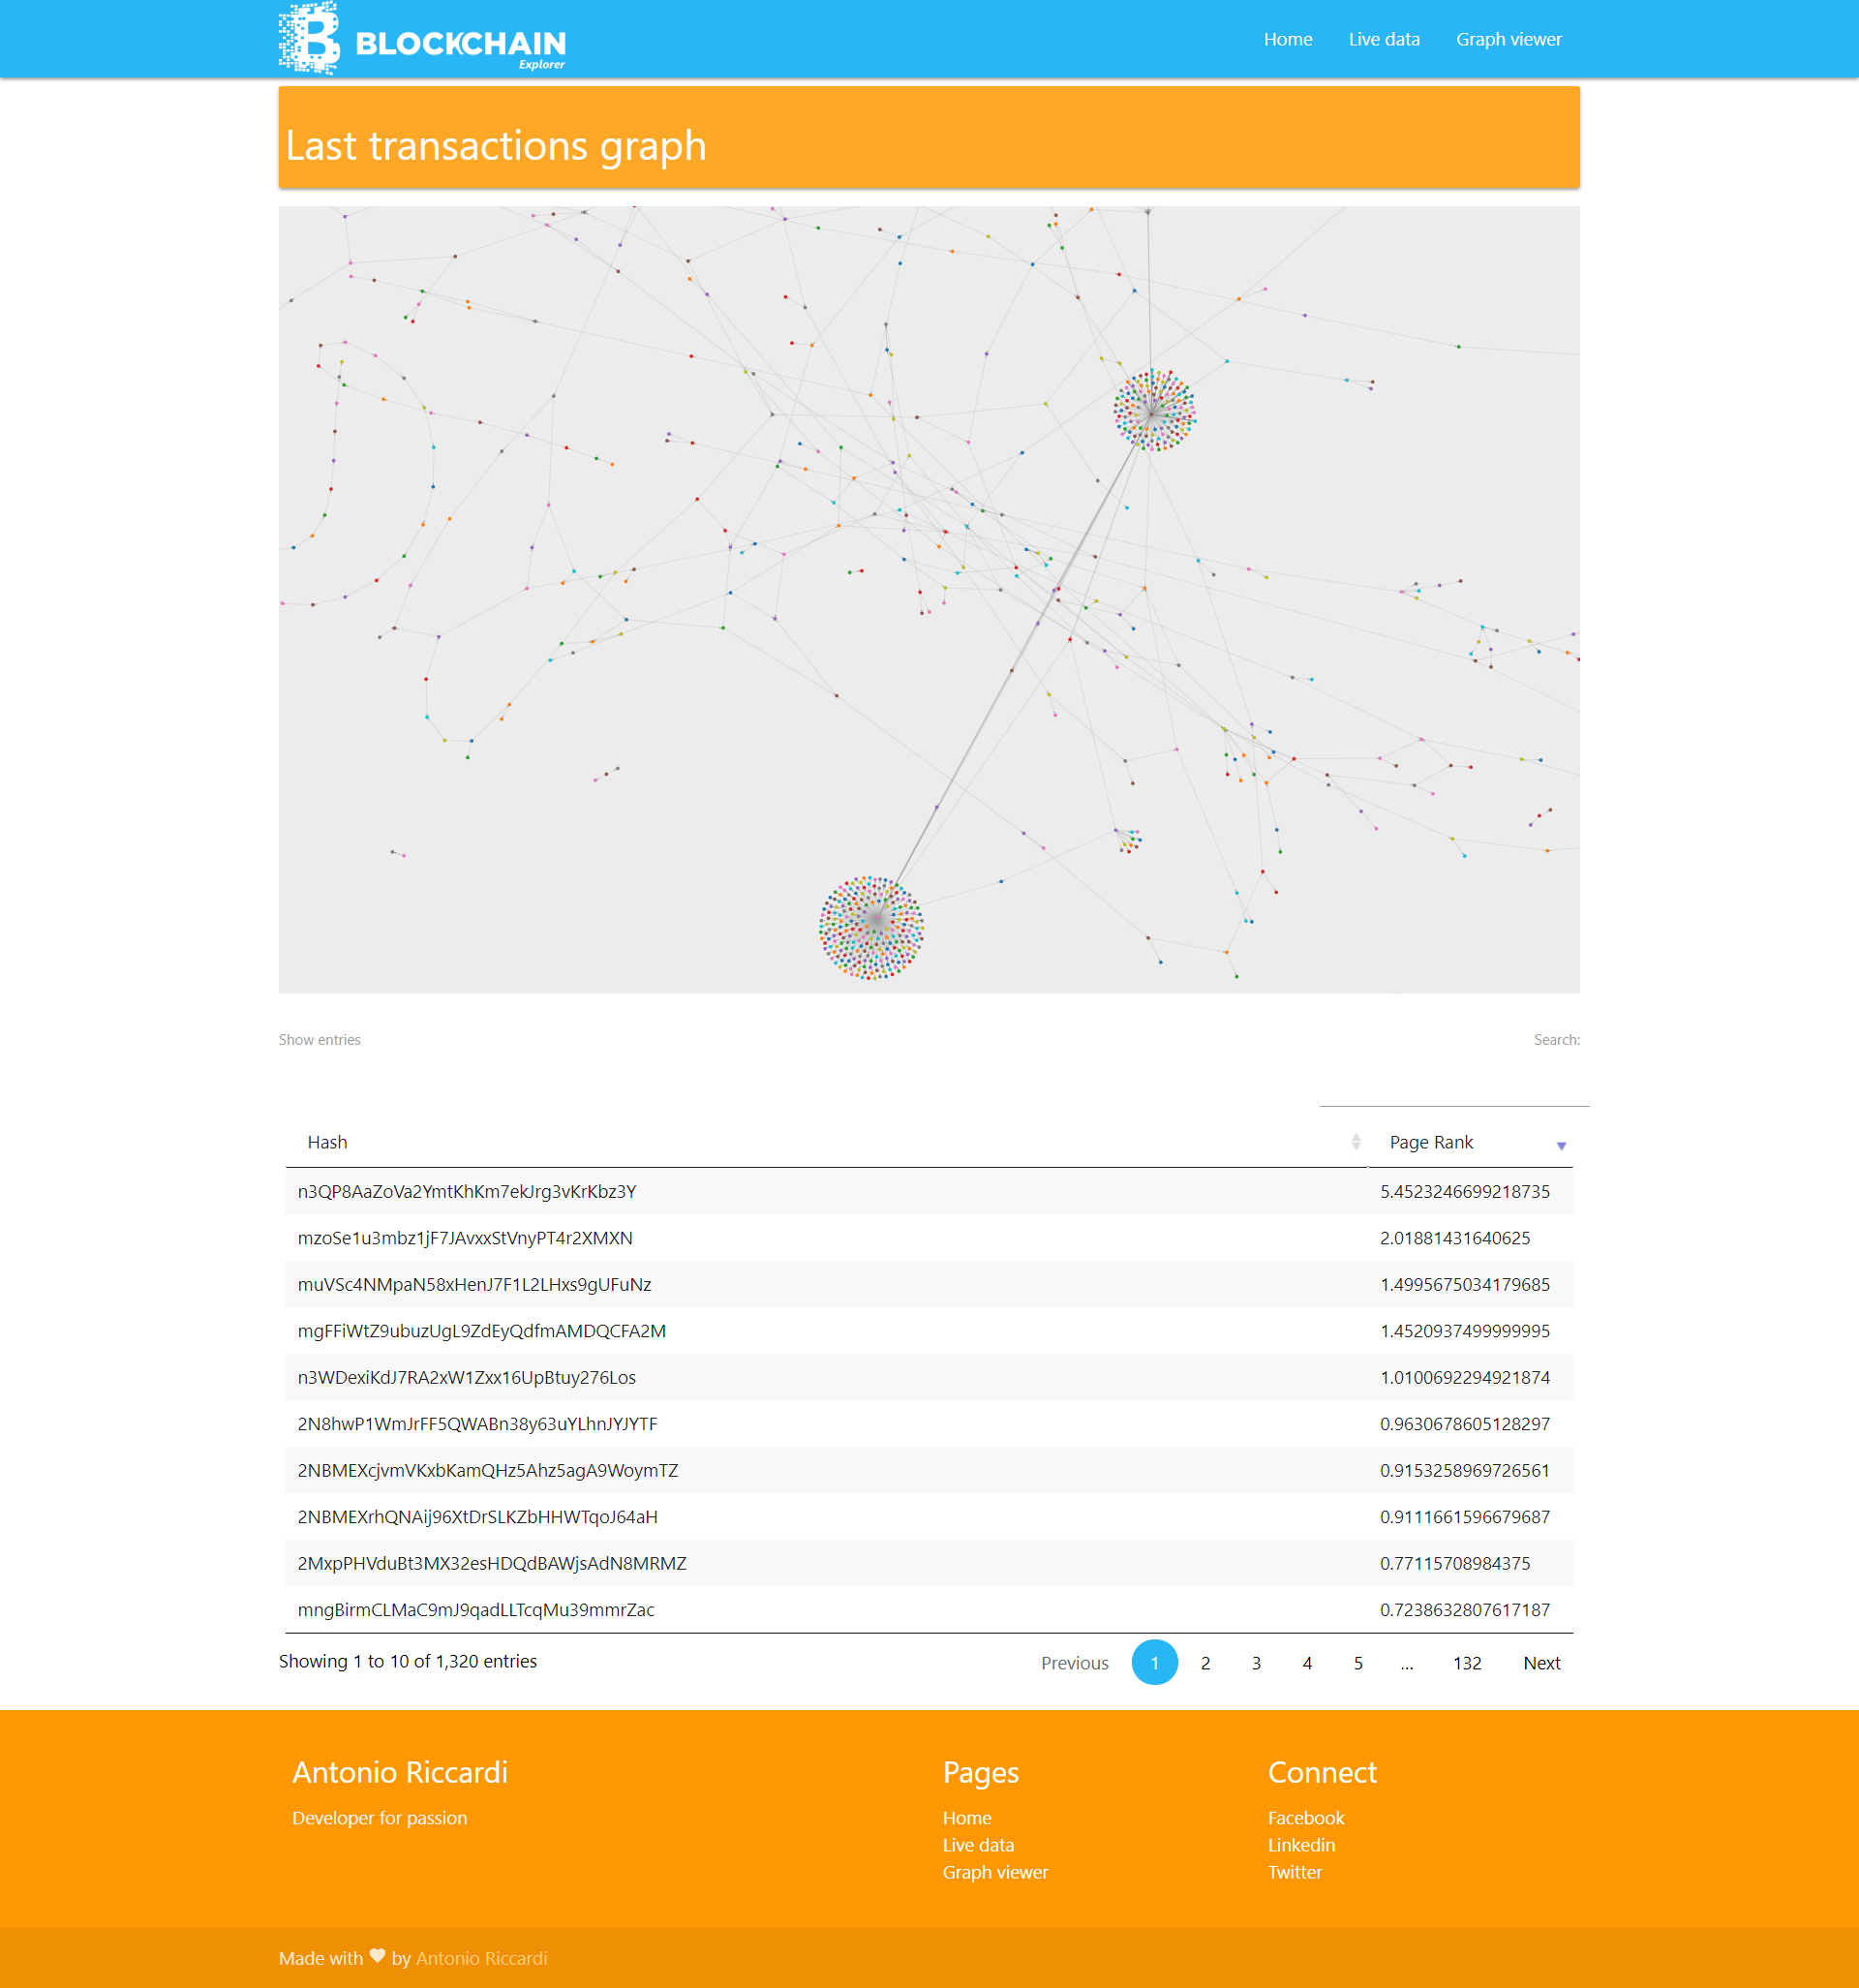
\includegraphics[width=\textwidth, height=0.65\textheight]{images/pageRankView.png}
	\caption{Visualizzazione intero grafo con calcolo del Page Rank.}
	\label{fig:graphPageBE}
\end{figure}
L'immagine \ref{fig:graphPageBE} mostra lo stato della blockchain all'interno della base dati del sistema tramite grafo orientato ed il valore del PageRank per ogni indirizzo hash calcolato dal sistema distribuito.
\\Tramite l'utilizzo del mouse, l'utente può navigare attraverso il grafo andando ad ingrandire per trovare un particolare indirizzo hash [\ref{fig:graph1BE}] oppure cercare una transazione ed ottenere i dati più significativi [\ref{fig:graph2BE}] semplicemente passando con il mouse sopra.
\begin{figure}[H]
	\centering
	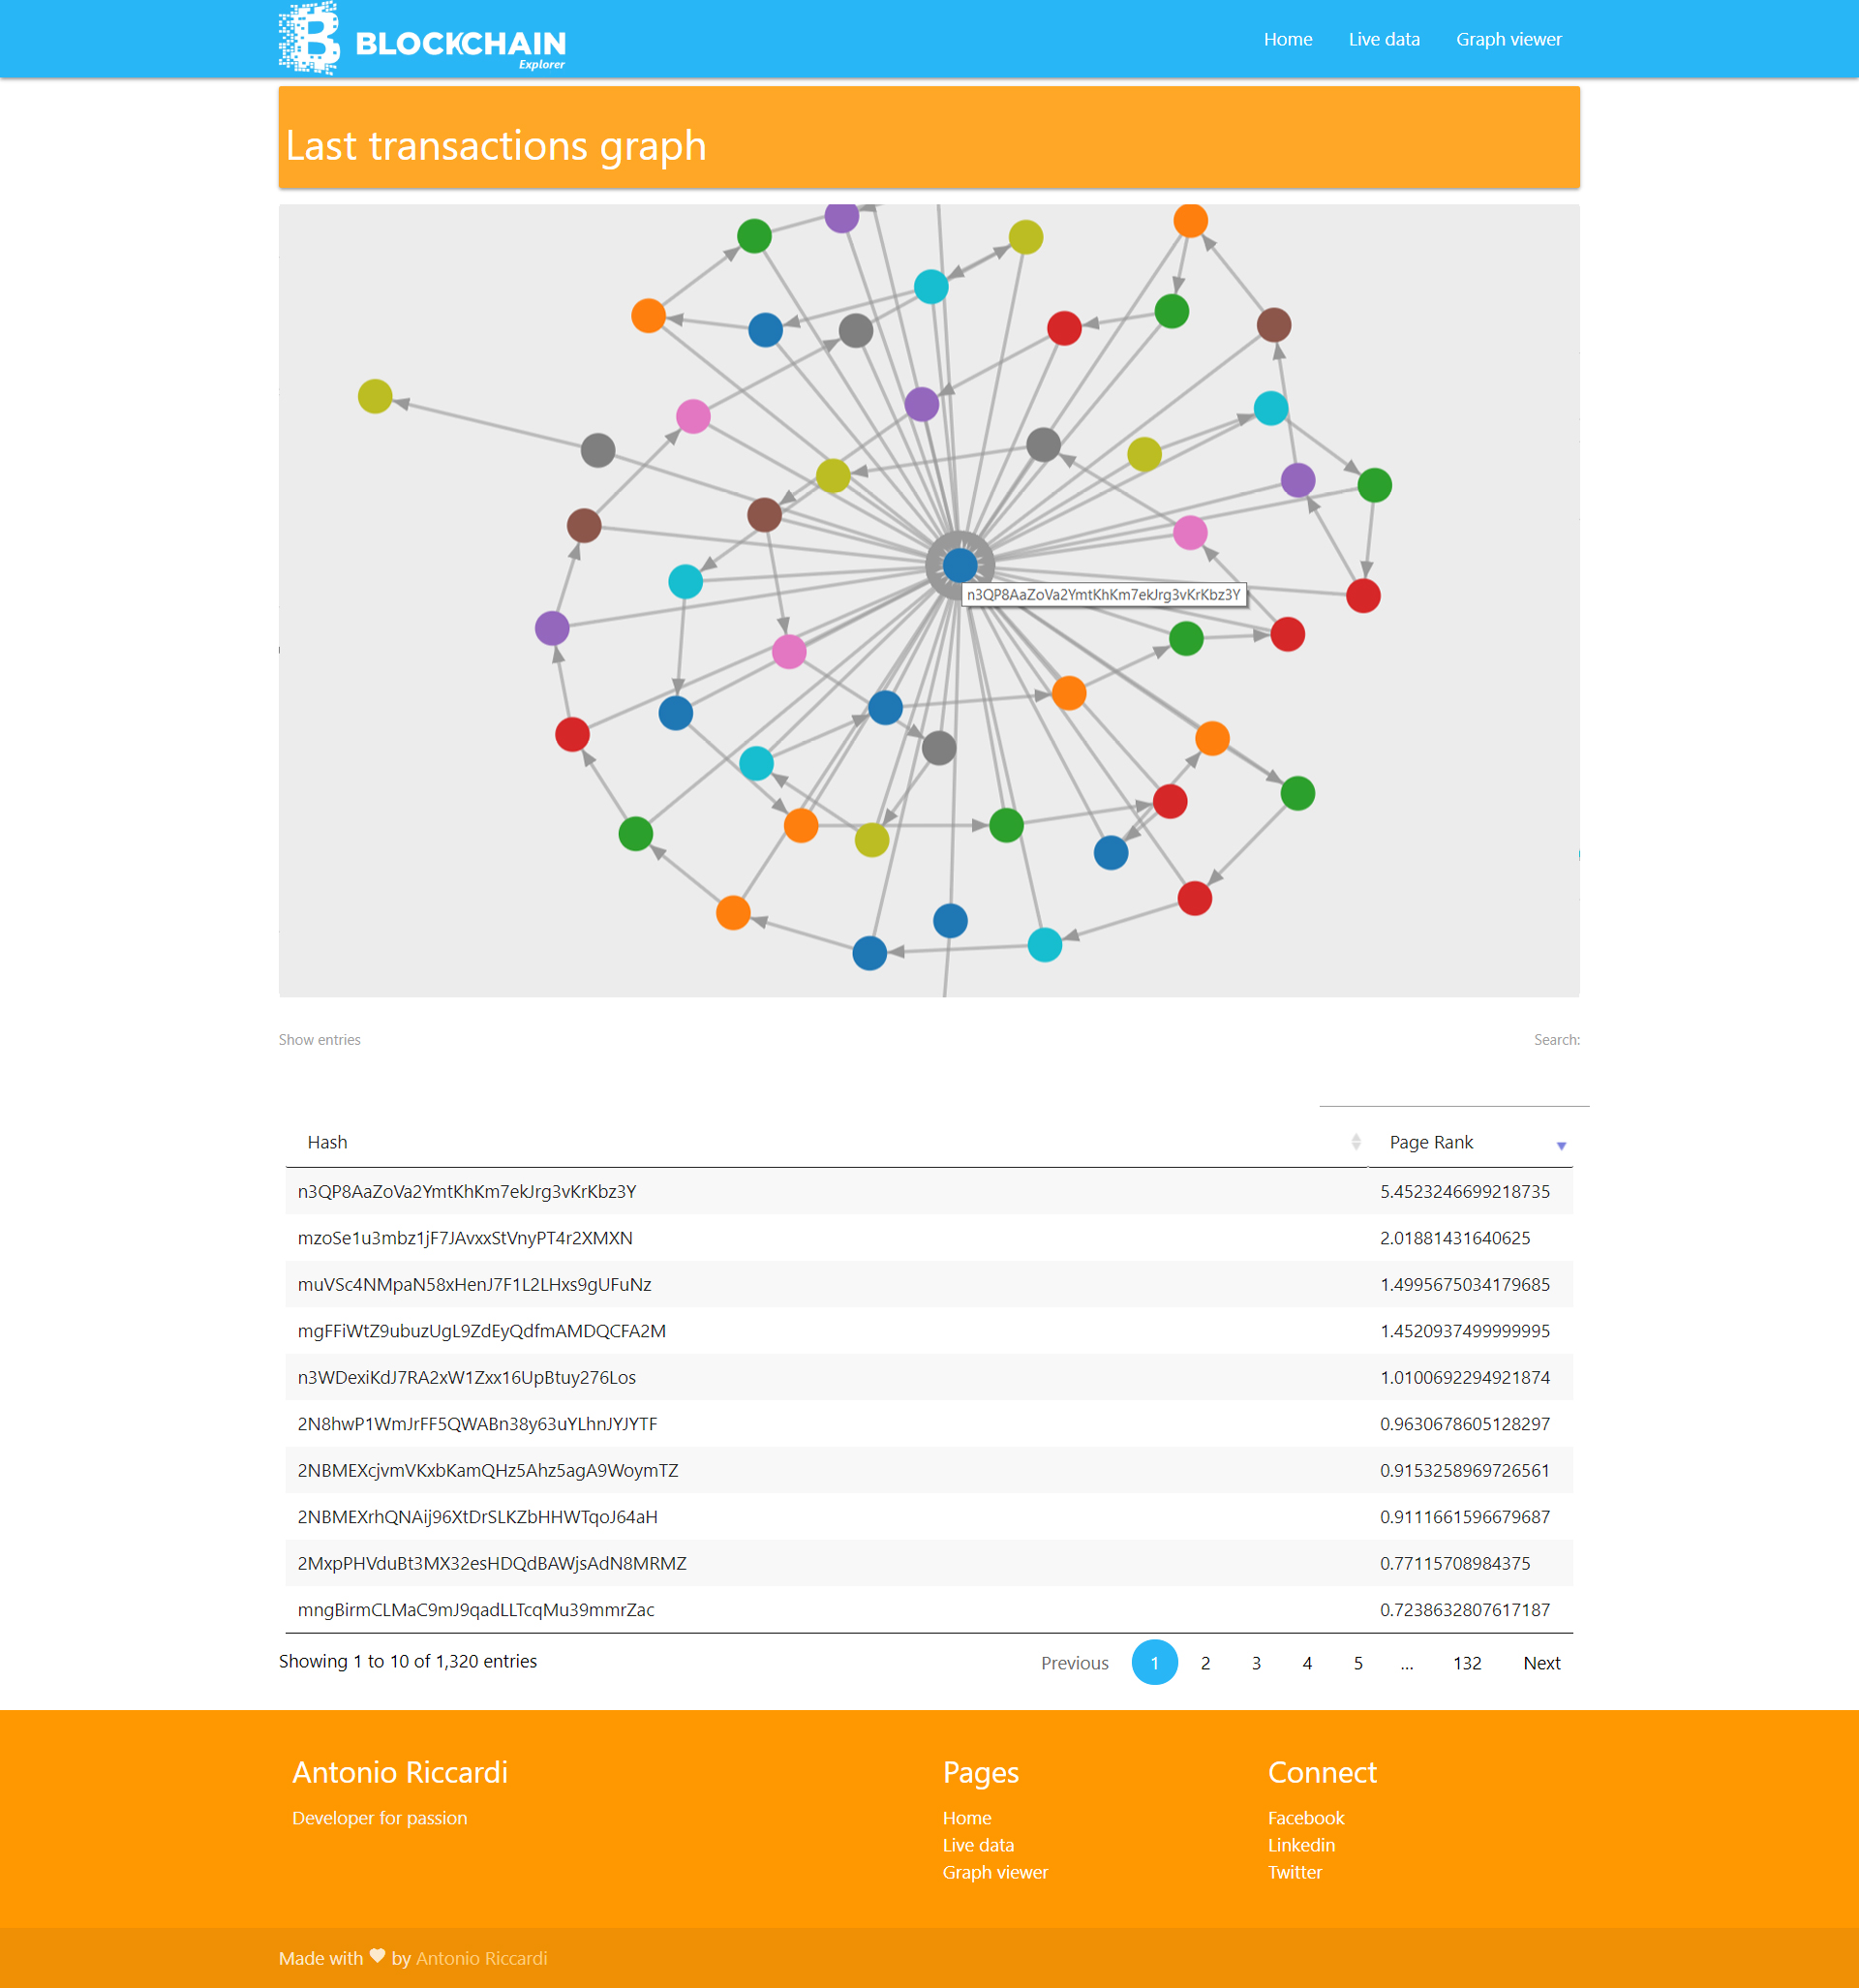
\includegraphics[width=\textwidth, height=0.70\textheight]{images/lastGraph-1.jpg}
	\caption{Dettaglio nodo centrale.}
	\label{fig:graph1BE}
\end{figure}
\begin{figure}[H]
	\centering
	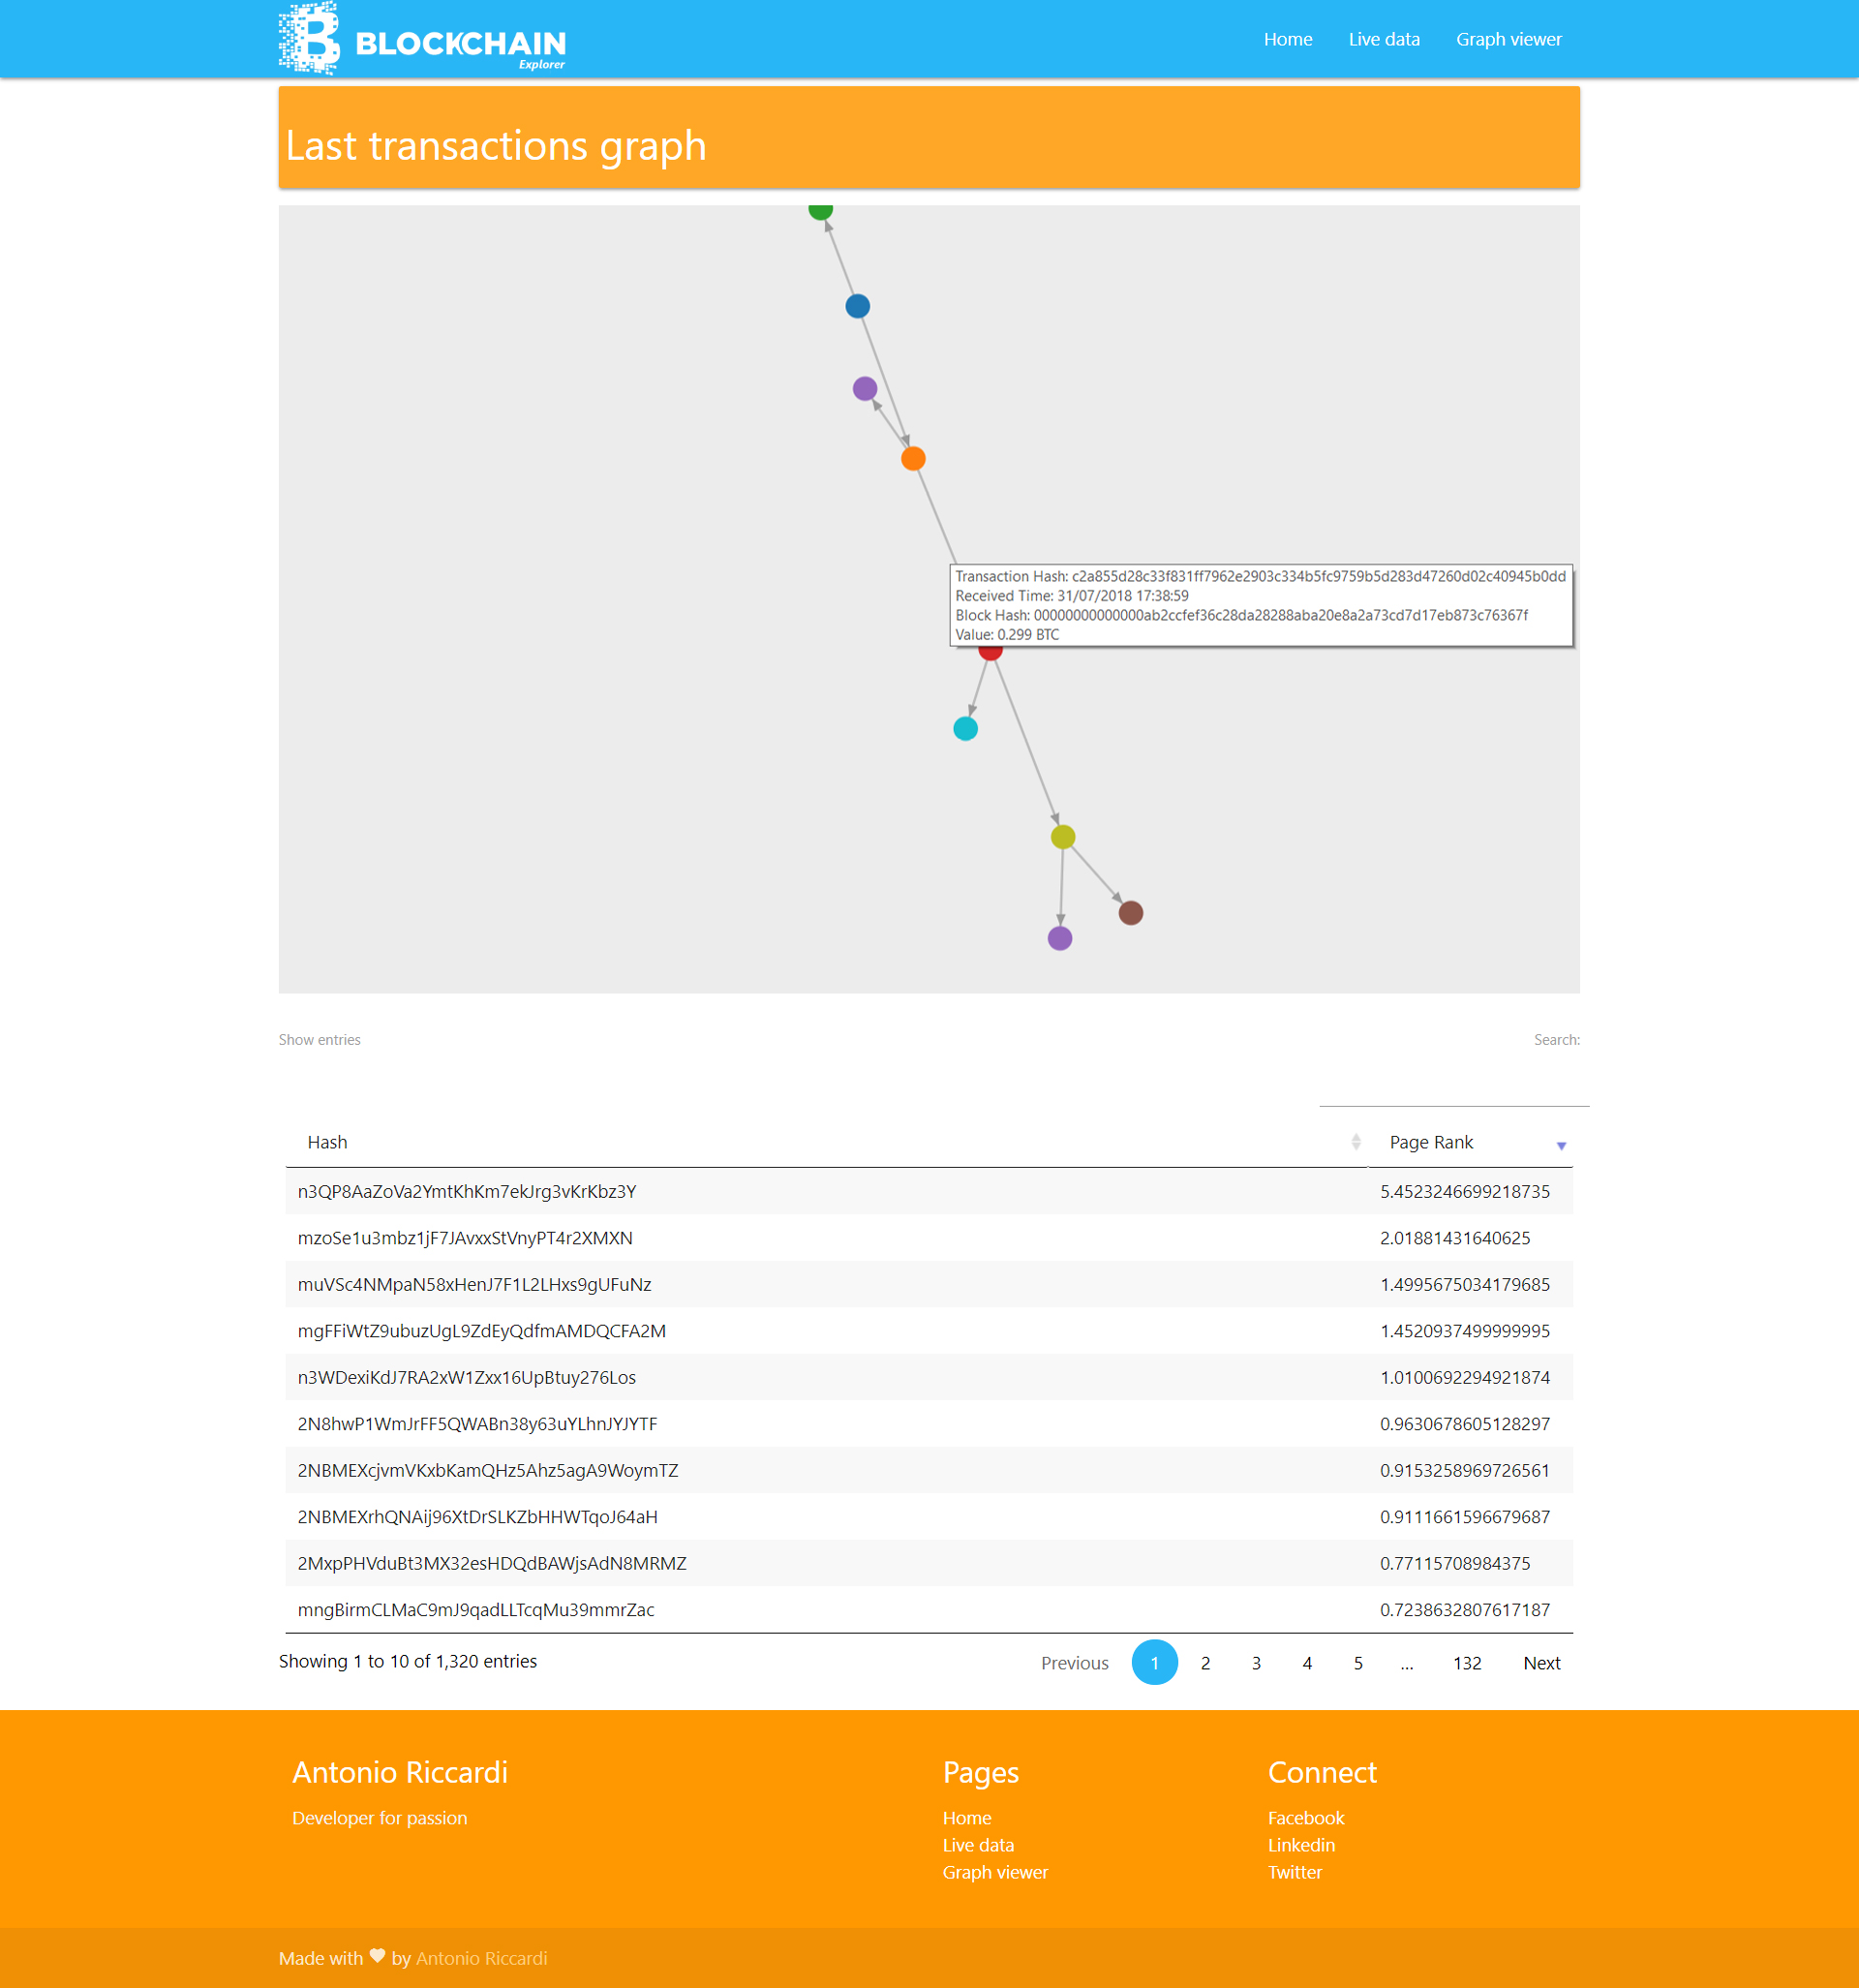
\includegraphics[width=\textwidth, height=0.70\textheight]{images/lastGraph-2.jpg}
	\caption{Dettaglio transazione all'interno del grafo.}
	\label{fig:graph2BE}
\end{figure}
Infine, è possibile ricercare hash all'interno della tabella del PageRank semplicemente cliccando con il tasto destro sul nodo all'interno del grafo. Questa funzionalità cercherà all'interno del database il valore del page rank associato al nodo e lo mostra nella tabella sottostante.
